%!TEX root = ../template.tex
%%%%%%%%%%%%%%%%%%%%%%%%%%%%%%%%%%%%%%%%%%%%%%%%%%%%%%%%%%%%%%%%%%%
%% introduction.tex
%%
%% Chapter with Introduction
%% REVIEWED by Diogo Gato 2022/03/29
%%%%%%%%%%%%%%%%%%%%%%%%%%%%%%%%%%%%%%%%%%%%%%%%%%%%%%%%%%%%%%%%%%%

%%TODO: Colocar Artigos Artigos Corretamente

\typeout{NT FILE introduction.tex}

\chapter{Introduction}
\label{cha:introduction}

\section{Context and Motivation} 
\label{sub:if_you_use_this_template} 

Over the past two decades, many governmental entities have implemented a wide array of policies aimed to reduce the CO\textsubscript{2} missions of the electricity sector by increasing the market penetration of renewable energy technologies \cite{OLD_3_GENERAL}. Due to this, there is an increase on the research of new, safe, and sustainable green power technologies, such as wind-based ones. The primary focus of renewable energy technologies research is to convert renewable resources into electrical energy to feed the utility grid or consumer loads \cite{OLD_1_SOLAR}.

Despite all the technologies that exist to assist the monitoring of renewable energy systems, failures in their assets are still one of the major problems that decrease the potential of those assets. “Ensuring that wind turbines perform at their optimal level over their lifetime (usually 20-25 years) costs around 25\% of the offshore installation” \cite{OLD_15_WIND}. Also, “technical faults that require unscheduled maintenance are increasingly important” and represent a large part of the total of failures on wind turbines \cite{OLD_18_WIND}.

This is where the CGI Renewable Management System (RMS) enters. Monitoring systems are essential to maintain optimal performance of renewable systems assets. With this master thesis work, we are trying to improve CGI RMS system by implementing a fault detection tool, to help our system clients in detecting possible failures soon and thus, improving the overall performance of their systems and reducing maintenance costs.


\section{Problem Definition} 
\label{sub:if_you_use_this_template} 

Renewable energy technologies, like wind turbines, are based in complex mechanic components that are subject to multiple external conditions. These external factors allied with the complexity and degradation of the components of wind turbines, may lead to failures in the assets that compose a power plant. These failures lead to downtimes in the production of energy to the grid and repairs, that cost money and resources to the owners of the power plants.

In wind farms, many failures of wind turbines are unpredictable. According to \cite{OLD_44_WIND} and \cite{OLD_18_WIND}, major faults in wind turbines that cause more than one day of downtime, only represent 25\% of all the failures that occur in a wind turbine. Despite this low percentage, these major faults are responsible for 95\% of the total downtime that occur in wind turbines.

A wind turbine is composed by complex components interconnected between them. The complexity of each component varies and consequently the mean time between failures (MTBF) and cost of repair of each one also changes. In \cite{OLD_55_WIND}, this is exactly what is analyzed, considering as a base a 2.3 MW onshore wind turbine. Considering the alarms history (by hours) from two years, it was recorded the failures duration for different assemblies. As a cost reference, we selected two of the variables that \cite{OLD_55_WIND} used: (i) the C0, that represents the cost of the non-delivery energy and (ii) the Cf (Cost of Failures), that represents the cost of failure of the component. With these variables presented before, in Figure 1.1, we present a chart from the data collected in Table 1 of \cite{OLD_55_WIND} and that correlates the number of hours of failure and the different costs (C0 and Cf) from each assembly that composes a wind turbine.

\begin{figure}[htbp]
	\centering
	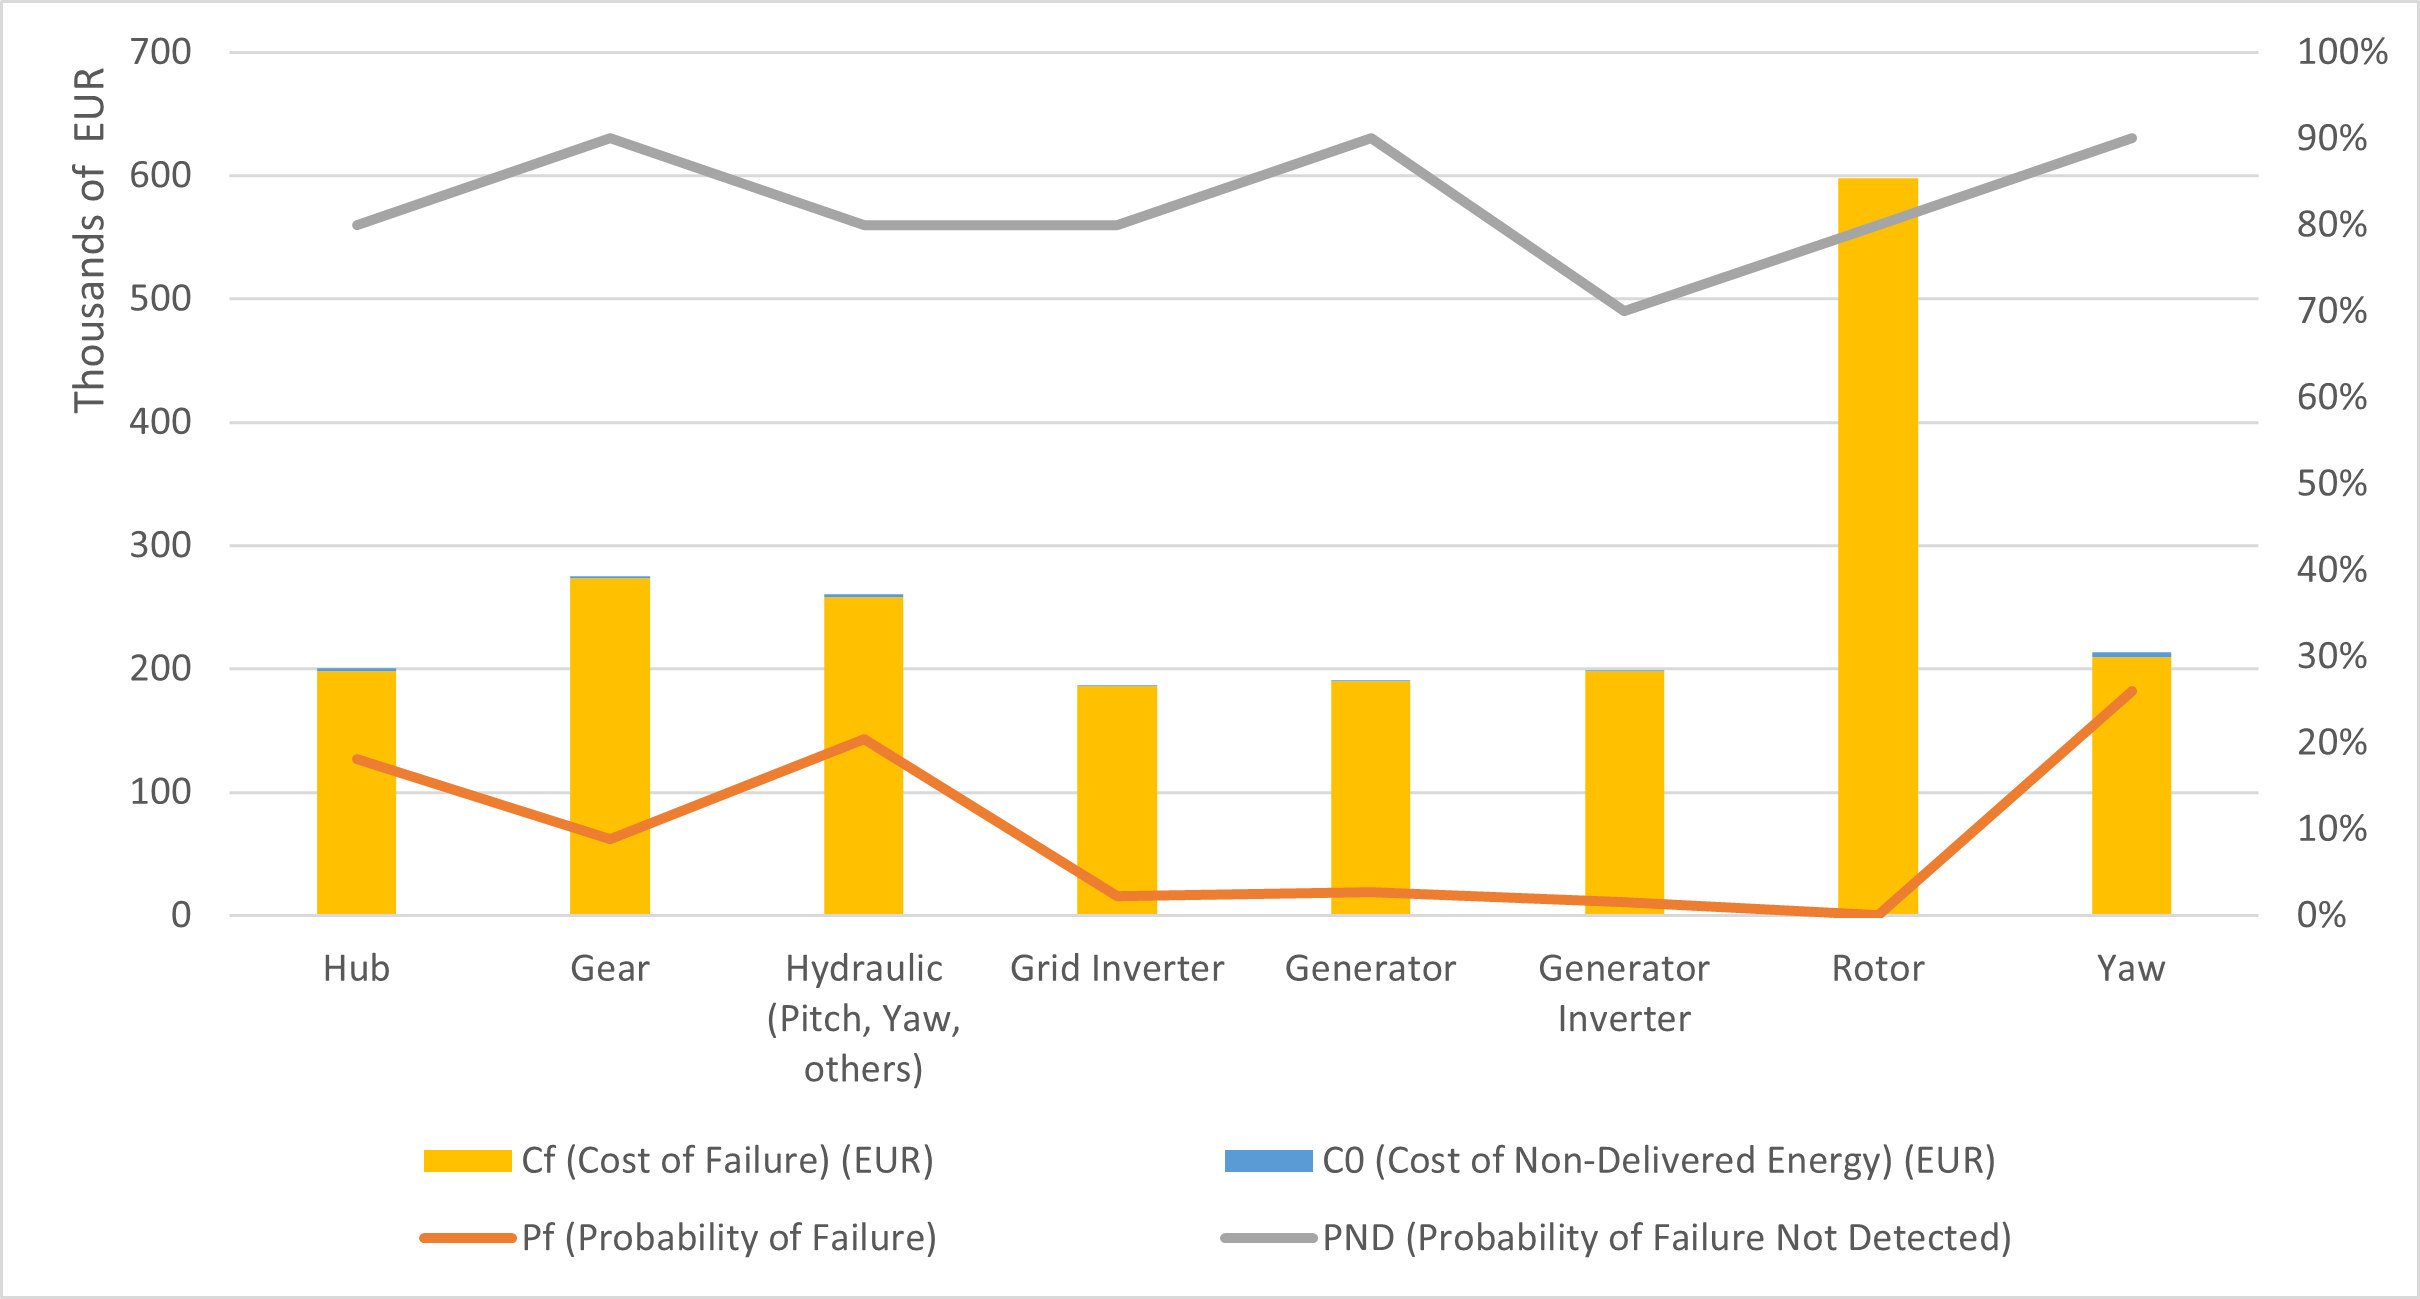
\includegraphics[scale=0.8]{Chapters/Figures/introduction_fig1.png}
	\caption{Costs of non-delivered energy and failure correlated with the Probability of Failure and Probability of Failure Not Detected for each component of a Wind Turbine. Data Source: \cite{OLD_55_WIND}}
	\label{fig:Figuras_Tree_silhouettes-vectorial}
\end{figure}

As we can see In Figure 1.1, the probability of failures that are not detected, in all key components that are represented, are in average above 80\% . Despite the fact of actual failures in the Rotor (that is the component that the total cost is higher) being almost 0\%, the next two components that have the higher cost of failure, Gear and Hydraulic failures, have a probability of failure of 9\%  and 20\%. The costs of these, two combined, surpasses the 500,000 €, that is a much higher cost compared to the costs of maintenance and monitoring of the components.

%TODO: FIX THE & Character

In \cite{OLD_53_WIND}, it is presented an analysis of the costs of failures in wind turbines, com-pared to the costs of a correct O&M (Operation and Maintenance) (including predictive maintenance). According to this study, the cost of O\&M during a 20-years lifetime in a 2 MW onshore wind turbine in a 200-MW project, is around 1.7M € and in a 4,14 MW offshore wind turbine in a 600-MW project, the cost is around 12.6M €. These costs were in addition to the cost for lost energy production during the failure and maintenance period.

“Proactive maintenance is expected to decrease downtime and the cost of failure, but the extent and frequency of needed maintenance is debatable” \cite{OLD_53_WIND}.

Further in this article, it is presented that “employing a condition monitoring system would result to savings of 190,000 € for a 3 MW wind turbine”. If no preventive maintenance is employed, the cost of the corrective maintenance is 436,299 €, whereas the “total O\&M cost would be 66,129 € if there are two preventive maintenance events per year per turbine in its entire life”, according to the average presented by O&M databases \cite{OLD_53_WIND}. This result in a total of 370,170 € profit, by using a predictive maintenance.

\section{Goals} 
\label{sub:if_you_use_this_template} 

To maximize energy production, increase availability, control energy losses and improve overall operational performance, CGI Renewable Management System (RMS) \cite{OLD_8} features an integrated set of tools. This master thesis study has the objective to improve this system, more particularly to study the base of the tool Failure Prediction from the Predictive module by using Artificial Intelligence. By extracting and studying the data available, our goal is to analyze all the steps needed to build a machine learning experiment, that will work as a foundation to predict faults in a wind turbine and to be used in the Failure Prediction tool, thus providing to the client a tool that predict exceptional situations and failures in the operation of renewable energies assets.

With the use of CGI RMS, we will have available real-time and historical data from real assets that exists on the field. With this data, we will be able to build a data-driven based method for fault detection with the help of machine learning algorithms. We will study, implement, and adapt supervised learning algorithms that are adequate to failure prediction, study the historical data available in CGI RMS from multiple signals and feed them to the previous referred algorithms. We will analyze the obtained results, comparing them against the historical data that we have available, so that we can check which algorithms and set of features are the more adequate to predict faults of multiple wind turbines. To conclude our work, we will then prepare these build models to be feed to the Failure Prediction tool available In CGI RMS.

To achieve this, we are going to divide the study of our thesis in five different scopes:

\begin{enumerate}
\item 
First, we are going to select the type of exceptional situations and failures in renewable energies assets we shall try to predict.

\item 
Then, we are going to study data so that we can identify the variables that allow us to predict such situations. These variables can be signals from the field and historical data events (like downtimes and faults that were registered) and we will do some previous analysis on the signals that may be related to each fault.

\item
We will perform some feature engineering, by using the Azure Machine Learning Studio built-in modules to analyze which features have more correlation with the fault events, building new features from the initial set of variables and to analyze our historical failure events that we have available to confirm that we have an unbalanced training set (since, naturally, the number of failures events is less that the normal operation events) and prepare a future step on balancing the training set for model training.

\item 
By using the features identified on the previous step, we are going to develop the machine learning models for each wind turbine fault, that can be integrated with CGI RMS to help to predict and classify the major failures according to the real-time data that the system monitors.

\item 
After our models are trained and we acquire an output from our experiments, we will analyze and present our conclusions of our built models and experiment steps, and present the future improvements that must be done in order to implement the Failure Prediction tool on CGI RMS.

\end{enumerate}


\section{Expected Contributions} 
\label{sub:if_you_use_this_template} 

With this thesis work, first we will improve the CGI RMS predictive module, by implementing the base experiment for our Failure Prediction tool that directly helps our clients reducing their repair costs and improving their assets performance and production.

Beyond the contribution to RMS, we will study and try to accomplish an improvement in one of the most interesting areas in today’s world: renewable energies. By using a set of theoretical studies on possible algorithms that may lead to the decrease of failures in renewable energy assets, we expect to put into practice these studies and develop the most correct machine learning models, that allied with a real-time monitoring system, improve the monitoring systems of renewable energies, and help the green energy producers to improve their production and reduce their repair costs.
Allying a powerful tool like a Failure Prediction with a real-time monitoring system, will put the renewable energy systems one step closer to a world with no need for polluting energy sources.